\chapter{Metody předzpracování a segmentace obrazu}

V této kapitole jsou podrobněji popsány vybrané metody předzpracování a segmentaci obrazu.
Na závěr kapitoly jsou uvedeny nejpoužívanější vyhodnocovací metriky.

\section{Unsharp Masking}

Unsharp masking je metoda zpracování obrazu, která se používá zaostření obrázku.

\begin{equation}
    I_{\text{sharp}} = I_{\text{original}} + k \cdot (I_{\text{original}} - I_{\text{blurred}})
\end{equation}

$I_{\text{original}}$ je původní obrázek, $I_{\text{blurred}}$ je rozmazaný obrázek. Nejčastěji se k rozmazání používá Gaussovský filtr. $k$ je koeficient, který určuje sílu efektu \cite{gQ8rTS6z7UD6hnlM}.

Byla použita implementace z knihovny PIL [citace].

\section{Binarizace}

Metody binarizace (nebo také thresholdingu) mají za úkol nalézt prahovou hodnotu, podle které se obraz jednoznačně rozdělí na dvě třídy. Tím se oddělí pozadí od popředí.

\begin{figure}[H]
    \centering
    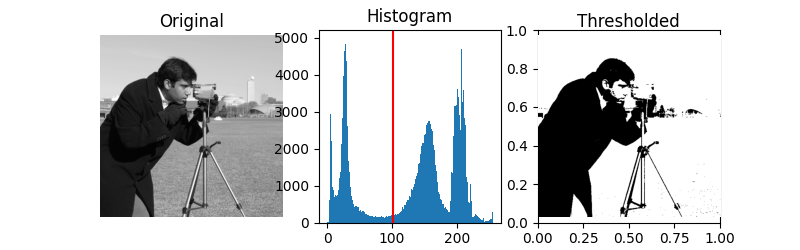
\includegraphics[width=\textwidth]{static/obrazky/thresholding_example.png}
    \caption{Binarizace obrazu Otsu metodou. Převzato z \cite{NEbfP3AWk7ALQfWN}.}
    \label{fig:thresholding}
\end{figure}

% Následuje popis několika metod binarizace.

\subsection{Otsu thresholding}

Metoda Otsu patří mezi nejpoužívanější metody binarizace. Algoritmus minimalizuje rozptyl uvnitř jednotlivých tříd.

\begin{equation}
    \sigma^2_w(t) = w_0(t)\sigma_0^2(t) + w_1(t)\sigma_1^2(t)
\end{equation}

$w_0(t)$ a $w_1(t)$ jsou pravděpodobnosti přiřazení pixelu do popředí resp. pozadí,
$\sigma_0^2(t)$ a $\sigma_1^2(t)$ jsou rozptyly tříd \cite{MopVANszPoidRZfR}.

Metoda je implementována v knihovně Scikit-image \cite{NEbfP3AWk7ALQfWN}.

\section{Morfologické operace}

Morfologické operace jsou základními nástroji pro zpracování a analýzu obrazů, které se používají k úpravě geometrických struktur v obraze. Řadí s k naprostému základu zpracování obrazu a proto zde uvedu pouze základní popis.

\subsection{Eroze}

Eroze je operace, která zmenšuje objekty v obraze. Používá se k odstranění malých objektů nebo šumu.

\subsection{Dilatace}

Dilatace je operace, která zvětšuje objekty v obraze. Používá se k vyplnění mezer nebo k propojení blízkých objektů.

\subsection{Otevření a uzavření}

Otevření je kombinace eroze a dilatace, která se používá k odstranění malých objektů a šumu. Uzavření je kombinace dilatace a eroze, která se používá k vyplnění mezer a propojení blízkých objektů.


\section{Watershed}

Algoritmus Watershed se používá k segmentaci objektů, které se dotýkají nebo překrývají.
Začne se umístěním markerů. Z každého takového bodu se pak obraz postupně „zaplavuje“, dokud se nesetkají dvě oblasti, které byly zaplavovány z různých markerů.
Nejčastěji se markery určí pomocí vzdálenostní transformace, kde se určí vzdálenost každého pixelu od nejbližšího pozadí.

\begin{figure}[H]
    \centering
    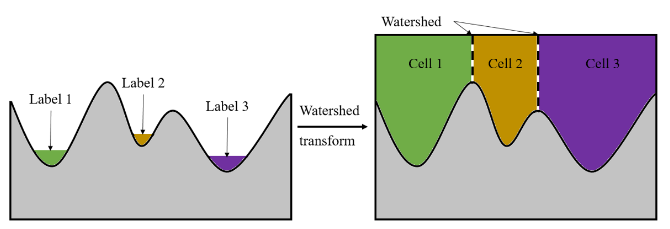
\includegraphics[width=\textwidth]{static/obrazky/watershed_process.png}
    \caption{Segmentace obrazu pomocí algoritmu Watershed. Převzato z [citace].}
    \label{fig:watershed}
    
\end{figure}
% https://www.researchgate.net/publication/349323744_Research_on_Distance_Transform_and_Neural_Network_Lidar_Information_Sampling_Classification-Based_Semantic_Segmentation_of_2D_Indoor_Room_Maps 


\section{Support Vector Machine}




\section{Vyhodnocovací metriky}

\subsection{Diceův-Sørensenův index}

Nejpoužívanější vyhdonocovací metrikou je Diceův-Sørensenův koeficient, známý též jako F1 skóre.

$$DSC = \frac{2 \times |A \cap B|}{|A| + |B|}$$

\subsection{Jaccardův index}



$$J = \frac{|A \cap B|}{|A \cup B|}$$